\subsubsection{Impact of Dual-Task Learning}
\label{sec:dual-task-result}


\begin{figure}[t]%[thbp]
\begin{center}
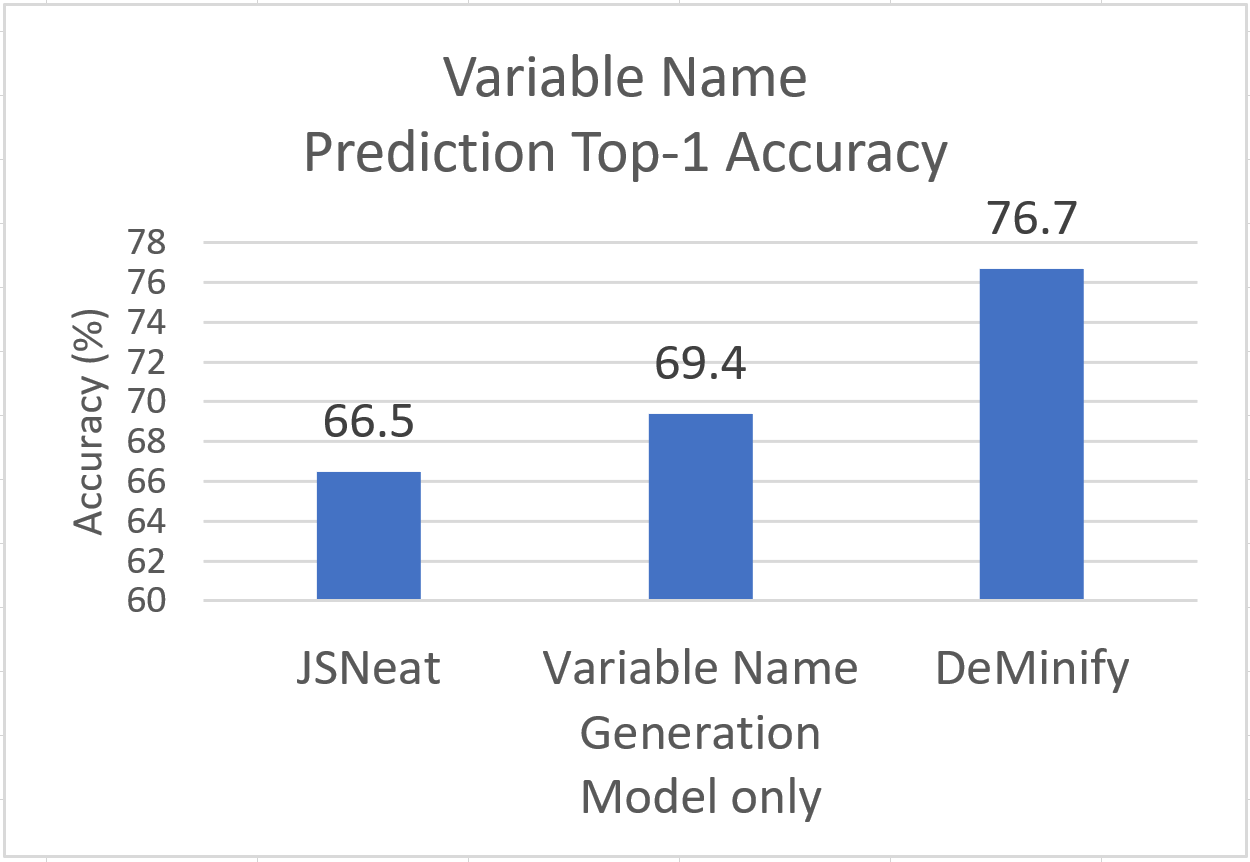
\includegraphics[width=2.1in]{figures/dual-task-result-11}
\vspace{-8pt}
\caption{RQ4. Dual-Task Learning on Name Prediction}
\label{dual-task-result-1}
\end{center}
\end{figure}

\begin{figure}[t]%[thbp]
\begin{center}
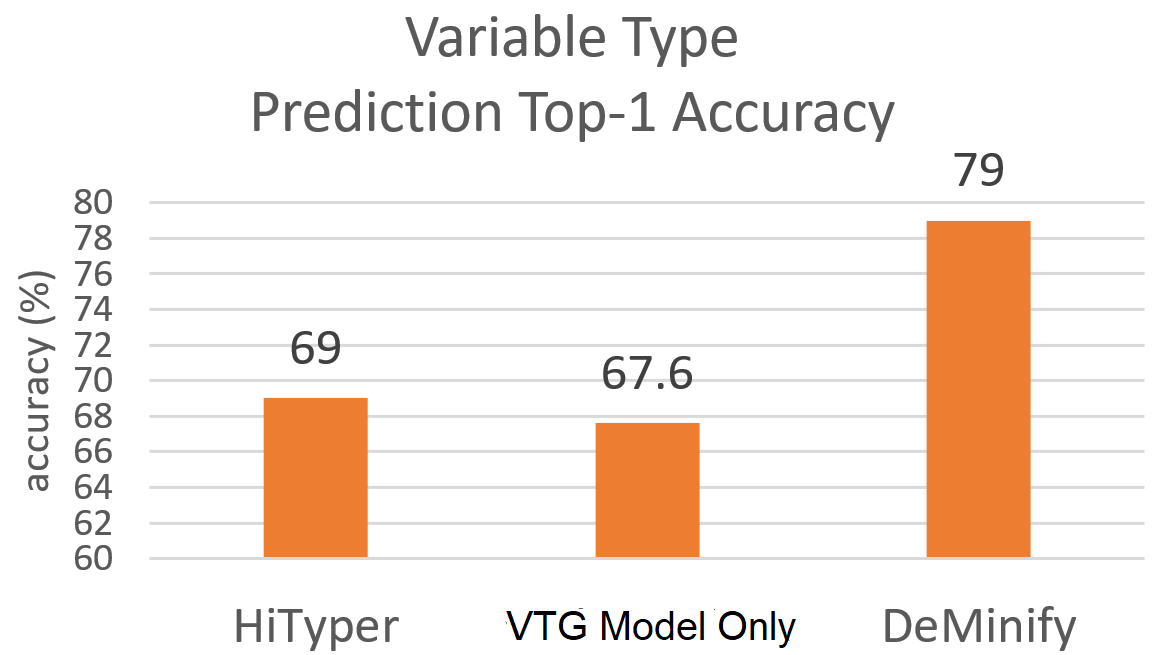
\includegraphics[width=2.1in]{figures/dual-task-result-22}
\vspace{-8pt}
\caption{RQ4. Dual-Task Learning on Type Prediction}
\label{dual-task-result-2}
\end{center}
\end{figure}

Figure~\ref{dual-task-result-1} shows the Top-1 accuracy in variable
name prediction when we removed the dual-task learning scheme and
measured only the accuracy of the variable name generation (VNG)
model.  As seen, without the impact from variable type generation
(VTG) via dual-task learning, VNG still performs better than the best
baseline, JSNeat (69.4\% versus 66.5\%). The drop in Top-1 accuracy
from {\tool} is 10.5\% (from 76.7\% downto 69.4\%). Similarly, as seen
in Figure~\ref{dual-task-result-2}, without the impact from VNG due to
the removal of the dual-task learning scheme, VTG performs slightly
worse than the best baseline HiTyper. The drop in Top-1 accuracy from
{\tool} is 14.4\%.  These results indicate the positive contribution to {\tool}
from our key ideas on the mutual impact of VNG and VTG via dual-task
learning.
